\documentclass{standalone}

\usepackage{tikz}

\begin{document}

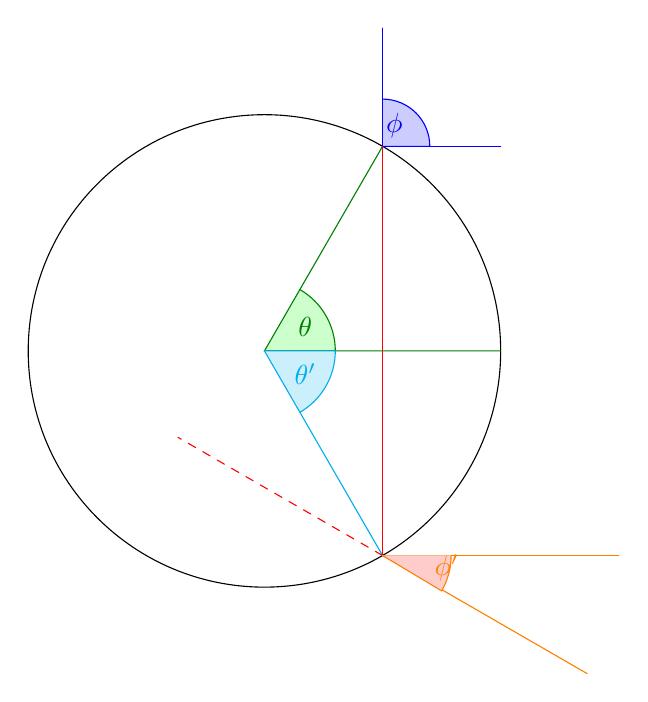
\begin{tikzpicture}[scale=3,cap=round]

    \colorlet{thetacolor}{green!50!black}
    \colorlet{phicolor}{blue}
    \colorlet{lcolor}{red}

    \draw (0,0) circle (1cm);

    \filldraw[fill=green!20,draw=thetacolor] (0,0) -- (3mm,0pt) arc(0:60:3mm);
    \draw (30:2mm) node[thetacolor] {$\theta$};

    \draw[thetacolor] (60:1cm) -- (0,0) -- (1cm, 0);

    \filldraw[fill=cyan!20,draw=cyan] (0,0) -- (3mm,0pt) arc(0:-60:3mm);
    \draw (-30:2mm) node[cyan] {$\theta'$};

    \draw[cyan] (-60:1cm) -- (0,0);

    \filldraw[fill=blue!20,draw=phicolor] (60:1cm) -- (0.7,0.866 cm) arc(0:90:2mm);
    \draw (60:1.1cm) node[phicolor] {$\phi$};

    \draw[phicolor] (60:1cm) -- +(0, 0.5);
    \draw[phicolor] (60:1cm) -- +(0.5cm,0);

    \draw[lcolor] (60:1cm) --  (-60:1cm);

    \draw[lcolor,dashed] (-60:1cm) -- +(-0.866,0.5);
    \draw[orange] (-60:1cm) -- +(0.866,-0.5);
    \draw[orange] (-60:1cm) -- +(1,0);

    \filldraw[fill=red!20,draw=orange] (-60:1cm) -- +(0.25,-.15) arc(-30:0:3mm);
    \draw (-50:1.2) node [orange] {$\phi'$};

\end{tikzpicture}

\end{document}